\documentclass[a4paper]{article}
\usepackage[utf8]{inputenc}
\usepackage[T1]{fontenc}
\usepackage[pdftex]{graphicx}
\usepackage{fancyhdr}
\usepackage{lscape}
\usepackage{color}
\usepackage{qtree}
\usepackage[english]{babel}
\usepackage{graphicx}
\usepackage[colorinlistoftodos]{todonotes}
\usepackage{listings}
\usepackage{color}
\usepackage{changepage}
\usepackage[margin=1in]{geometry}
\definecolor{codegreen}{rgb}{0,0.6,0}
\definecolor{codegray}{rgb}{0.5,0.5,0.5}
\definecolor{codepurple}{rgb}{0.58,0,0.82}
\definecolor{backcolour}{rgb}{0.95,0.95,0.92}
\usepackage[parfill]{parskip}

 \lstdefinestyle{mystyle}{
 	backgroundcolor=\color{backcolour},   
 	commentstyle=\color{codegreen},
 	keywordstyle=\color{magenta},
 	numberstyle=\tiny\color{codegray},
 	stringstyle=\color{codepurple},
 	basicstyle=\footnotesize,
 	breakatwhitespace=false,         
 	breaklines=true,                 
 	captionpos=b,                    
 	keepspaces=true,                 
 	numbers=left,                    
 	numbersep=5pt,                  
 	showspaces=false,                
 	showstringspaces=false,
 	showtabs=false,                  
 	tabsize=2
 }
 
\lstset{
	style=mystyle,
	inputencoding=utf8,
	extendedchars=true,
	literate={á}{{\'a}}1 {ã}{{\~a}}1 {é}{{\'e}}1,
	escapechar=\&
}
\title{Algorithmique et structures de données : Mission 2}
\date{18 octobre 2014}
\author{Groupe 1.2: Ivan Ahad - Jérôme Bertaux - Rodolphe Cambier \\ 
	Baptiste Degryse - Wojciech Grynczel - Charles Jaquet}



\begin{document}
\maketitle



Rapport écrit par Ivan Ahad et Rodolphe Cambier

\subsection*{Introduction}

L'objectif de cette mission est de créer un programme qui prend en entrée une expression analytique et qui retourne la dérivée de celle-ci, grâce à l'utilisation d'arbres binaires. 

\subsection*{Fonctionnement}

Le programme lit le fichier avec les expressions à résoudre et convertit les lignes du fichier en un ArrayList: 
\begin{lstlisting}[language=Java]
ArrayList<String> expressions = ReadWrite.mRead("expression.txt");
\end{lstlisting}

Il traite ensuite chaque élément de l'ArrayList indépendamment:
\begin{lstlisting}[language=Java]
for (String expression : expressions)
\end{lstlisting}

Pour chaque expression (élément de l'ArrayList), il va transformer la ligne de texte en un FormalExpressionTree, un arbre binaire qui va contenir les expression afin qu'elles soient traitables par la suite. Cela sera réalisé lors de la création de l'arbre, quand le constructeur de\textit{ FormalExpressionTreeImpl} appelle la fonction \textit{parse}.
\begin{lstlisting}[language=Java]
FormalExpressionTree fet = new FormalExpressionTreeImpl(expression);
\end{lstlisting}
						
Une fois transormées en arbre, les expressions mathématiques vont êtres dérivées en appelant la fonction \textit{derive}, de la classe \textit{Calculator} sur l'abre représentant l'expression mathématique à dériver. Cette fonction va traiter l'élément du root, et va s'appeler récursivement sur chacun des enfants du root, de sorte que tout l'arbre soit traité. A chaque étape, il remplit un nouvel arbre, avec la dérivée de l'expression de départ qu'il retourne finalement.

\begin{lstlisting}[language=Java]

	public static LinkedBinaryTree<String> derive(LinkedBinaryTree<String> t){
		LinkedBinaryTree<String> t2=null;		
		if(t.element().equals("+"))
			t2= new LinkedBinaryTree<String>("+",derive(t.leftTree()),derive(t.rightTree()));			
		else if(t.element().equals("-"))
			t2= new LinkedBinaryTree<String>("-",derive(t.leftTree()),derive(t.rightTree()));
		
		[...]
		
		else
			System.out.println("element inconnu : "+ t.element());		
		return t2;	
	}
\end{lstlisting}


Finalement, l'arbre de départ ainsi que le nouvel arbre représentant sa dérivée seront imprimés.	

\subsection*{Choix d'implémentations, optimisations}

LA fonction \textit{parse} de la classe \textit{FormalExpressionTreeImpl} se base fortement sur l'hypothèse simplificatrice des expression parenthésées. On se base en effet sur la fermeture d'une parenthèse pour conclure que les deux opérations précédentes (variable \textit{operands})doivent être liées dans un arbre avec comme racine l'opérateur correspondant (variable \textit{operators})et ainsi de suite récursivement: 

\begin{lstlisting}[language=Java]
if (token == ')') {
right = (LinkedBinaryTree) operands.pop();
left = (LinkedBinaryTree) operands.pop();
	[...]
LinkedBinaryTree lbt = new LinkedBinaryTree(operators.pop()+ "", left, right);
	[...]
operands.push(lbt);
}
\end{lstlisting}

Le rajout des fonctions exp et log se ferait de manière similaire aux fonctions cos et sin, avec un cas particulier dans la fonction  \textit{parse} et le calcul adapté dans la classe \textit{Calculator}. Notre implémentation permet donc le rajout de toute fonction voulue, simplement en l'insérant dans l'arbre et en la traitant de manière adaptée dans la classe \textit{Calculator}.

\subsection*{UML}

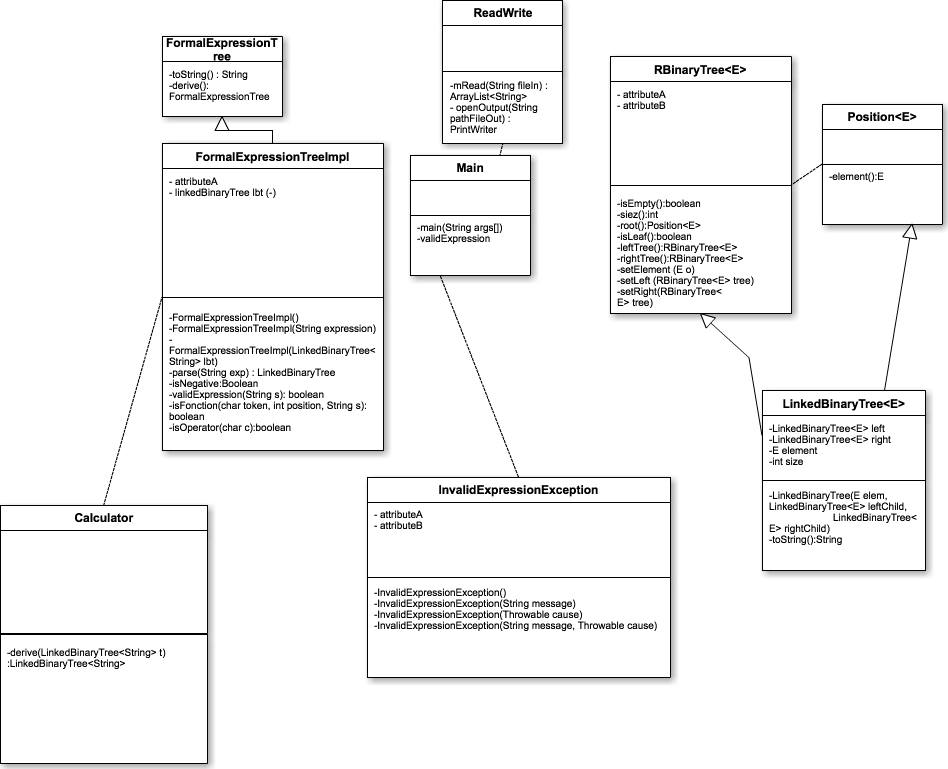
\includegraphics[scale=0.5]{uml}

\end{document}